\documentclass[10pt]{article}
\textheight=9.25in \textwidth=7in \topmargin=-.75in
 \oddsidemargin=-0.25in
\evensidemargin=-0.25in
\usepackage{url}  % The bib file uses this
\usepackage{graphicx} %to import pictures
\usepackage{amsmath, amssymb, bbold}
\usepackage{theorem, multicol, color}
\usepackage{gfsartemisia-euler} % best font in da game
\usepackage{tikz} % Graphs and other graphics

\setlength{\intextsep}{5mm} \setlength{\textfloatsep}{5mm}
\setlength{\floatsep}{5mm}
\setlength{\parindent}{0em} % new paragraphs are not indented
\setcounter{MaxMatrixCols}{20}
\usepackage{caption}
\captionsetup[figure]{font=small}


%%%%  SHORTCUT COMMANDS  %%%%
\newcommand{\ds}{\displaystyle}
\newcommand{\Z}{\mathbb{Z}}
\newcommand{\1}{\mathbb{1}}
\newcommand{\arc}{\rightarrow}
\newcommand{\R}{\mathbb{R}}
\newcommand{\N}{\mathbb{N}}
\newcommand{\Q}{\mathbb{Q}}
\renewcommand{\P}{\mathbb{P}}
\newcommand{\E}{\mathbb{E}}
\newcommand{\blank}{\underline{\hspace{0.33in}}}
\newcommand{\qand}{\quad and \quad}
\renewcommand{\stirling}[2]{\genfrac{\{}{\}}{0pt}{}{#1}{#2}}
\newcommand{\dydx}{\ds \frac{d y}{d x}}
\newcommand{\ddx}{\ds \frac{d}{d x}}
\newcommand{\dvdx}{\ds \frac{d v}{d x}} 

%%%%  footnote style %%%%

\renewcommand{\thefootnote}{\fnsymbol{footnote}}

\pagestyle{empty}

\begin{document}

\begin{flushright}
Chandler Justice - A02313187
\end{flushright}
\noindent \underline{\hspace{3in}}\\
\textbf{MATH5620:} Homework \#3 \\
\textbf{Due:} A long time ago\\

\textbf{Problem 1:} For the example problem
\[u''(x) = f(x)\]
With $f(x) = \cos\left(\frac{3\pi}{2}x\right)$ with boundary conditions $u(0) = 0$ and $u(1) = 1$, compute a computational convergence study to verify the order of accuracy analysis. Use the sequence of $h$ values
\[h_i = \left\{\frac{1}{8}, \frac{1}{16}, \frac{1}{32}, \cdots, \frac{1}{2^8} \right\}\]

\textbf{Solution 1:} I wrote the following class to facilitate the computation and accuracy analysis
\begin{verbatim}
class FiniteDifference:


    def __init__(self, left_endpoint: float, right_endpoint: float, num_points: int, 
    fx: Callable, exact_function: Callable, h_val = None) -> None:
        # initialize data

        self.function_values = []
        self.interval_points = []
        self.h = 0
        self.approx_solutions = []
        self.matrix = np.array 

        self.left_endpoint = left_endpoint
        self.interval_points.append(left_endpoint)
        self.right_endpoint = right_endpoint
        self.interval_points.append(right_endpoint)
        self.num_points = num_points 

        self.mesh_interval = self.determine_mesh_interval()
        self.create_interval_points()
        
        self.fx = fx 
        self.exact_function = exact_function

        if h_val == None:
            self.h = 1 / (1 + self.mesh_interval)
        else:
            self.h = h_val

    def determine_mesh_interval(self):
        return (self.right_endpoint - self.left_endpoint) / (self.num_points - 1)


    def create_interval_points(self):
        curr_val = self.left_endpoint + self.mesh_interval
        for i in range(1, self.num_points - 1):
            self.interval_points.insert(i, curr_val)
            curr_val += self.mesh_interval
   

    def construct_matrix(self):
        k = [np.ones(self.num_points-1),-2*np.ones(self.num_points),np.ones(self.num_points-1)]
        offset = [-1,0,1]
        self.matrix = diags(k,offset).toarray()


    def create_approximate_solutions(self):
        self.function_values.append(self.left_endpoint)

        # use 2nd order finite difference approx 
        for i in range(1,self.num_points - 1):
            second_difference = (1 / self.h**2) * (self.fx(self.interval_points[i - 1]) \
            - (2 * self.fx(self.interval_points[i])) + self.fx(self.interval_points[i + 1]))
            self.function_values.append(second_difference)
        self.function_values.append(self.right_endpoint)


    def solve_linear_system(self):
        func_vals = np.array(self.function_values).transpose()
        self.approx_solutions = np.linalg.solve(self.matrix, func_vals)


    def solve(self):
        self.construct_matrix()
        self.create_approximate_solutions()
        self.solve_linear_system()


    def compute_global_error(self):   
        exact_solutions = []
        error_at_term =  0
        # find exact solutions
        for point in self.interval_points:
            exact_solutions.append(self.exact_function(point))
        # find error between approx soln and exact soln
        for i, solution in enumerate(exact_solutions):
            error_at_term += (abs(self.approx_solutions[i] - solution)**2)
        # compute l2-norm
        l2_norm = math.sqrt(error_at_term)
        return l2_norm
\end{verbatim}
\newpage
\textbf{Question 2:} Using Matplotlib graph the solutions obtained in the computational convergence study

I wrote the following code to graph the behavior of my approximation:
\begin{verbatim}
def display_data(solutions):
    plt.plot(solutions)
    plt.show()
\end{verbatim}
As you can see, using Matplotlib makes life very easy. Here is the graph obtained from my program

\begin{figure}[h!]
    \centering
    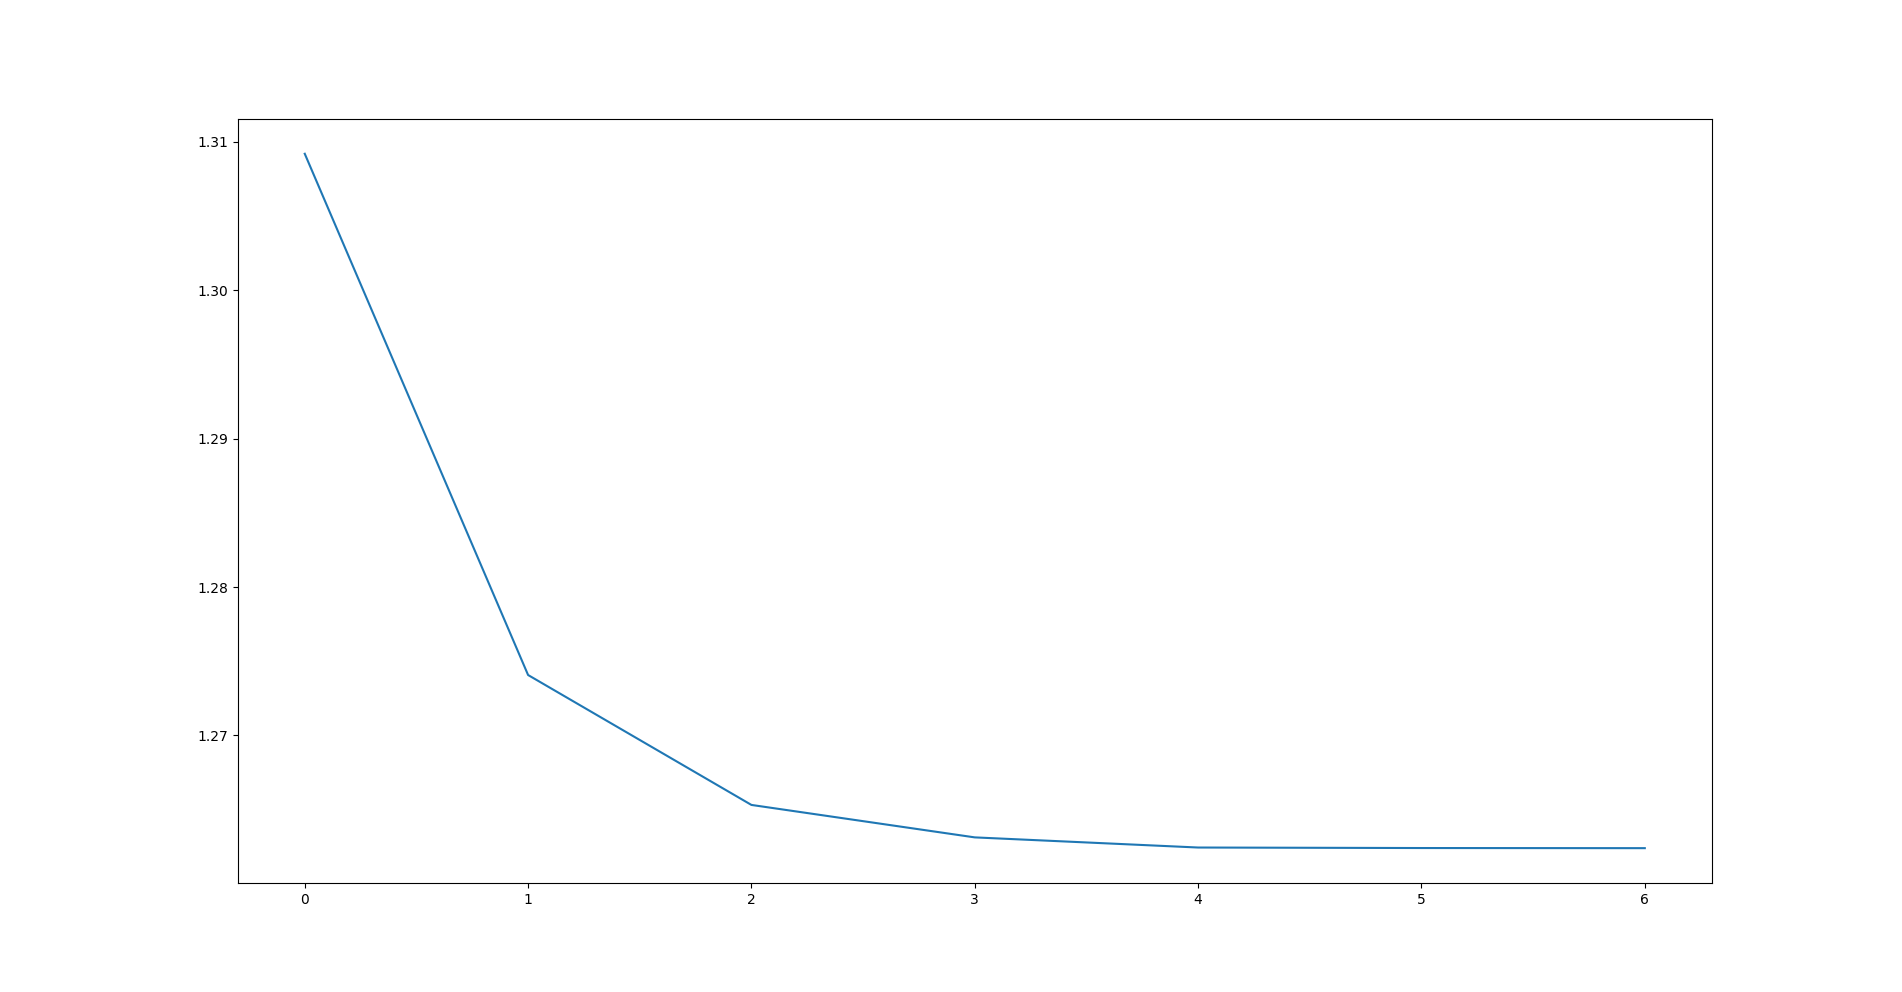
\includegraphics[scale=0.3]{Figure_1.png}
\end{figure}

\textbf{Question 3:} The finite difference scheme can be changed by including an alternative difference quotient. Use the code written in Assignment/Homework 1 to produce coefficients for a fourth order derivative approximation of $u''$. Use a centered difference quotient. Describe problems that occur at the boundaries of the domain. How does the alternate method incorporate the boundary conditions? If a reflection condition is applied at the boundary points, determine if this effects the accuracy of the approximation.\\

\textbf{Solution 3:} My code for homework 1 did not produce accurate results, so I opted to use the solution posted on github. Upon comparing results I found that the disparity between these methods to be huge. Here is a sample of the results obtained

\verb|4th order finite difference: [-0.16666715 -0.33333429 -0.50000189 -0.66666865 -0.83333432]|\\
\verb|4th order finite difference (hw1 soln): [ 10.66666667 -42.66666667  64. -42.66666667  10.66666667]|

The results are consistent, they are just the incorrect magnitude, implying that some scaling would produce a more accurate comparison\\

\textbf{Question 4:} Use your code from Assignment/Homework 1 to produce a fourth order difference that stays within the domain at the boundaries and use the foruth order central difference at points where possible. Discuss how the matrix structure is effected. What advantages are there to using the Jacobi iteration method over a Gaussian elimination approach?\\

\textbf{Solution 4:} In a Gaussian approach, the soltuion is obtained from all available data available at computation, whereas a Jacobi method relies solely on data available at initialization. This means for some functions the Guassian method might produce divergant results while the jacobi method will produce stable results. 

\noindent \underline{\hspace{3in}}\\

\end{document}

